%% 06_experimental_results.tex -- Experimental Evaluation and Convergence Analysis
%% -----------------------------------------------------------------------------

\chapter{Experimental Results}

\section{Experimental Configuration}
To validate the Genetic Algorithm's optimization capabilities on the 960-session class scheduling benchmark, we conduct systematic evolutionary runs under the hyperparameter configuration detailed in Table~\ref{tab:ga_hyperparams}.

\begin{table}[H]
  \centering
  \small
  \caption{Genetic Algorithm Hyperparameter Settings}
  \label{tab:ga_hyperparams}
  \begin{tabularx}{\linewidth}{L{5.0cm} C{3.0cm} X}
    \toprule
    \rowcolor{PrismHeader}
    \color{PrismWhite}\textbf{Hyperparameter} & 
    \color{PrismWhite}\textbf{Value} & 
    \color{PrismWhite}\textbf{Rationale / Purpose} \\
    \midrule
    Population Size ($N_{pop}$) & 40 -- 80 & Balances population diversity against per-generation computation time. \\
    Generations ($G$) & 50 -- 150 & Sufficient iterations to observe constraint decay and fitness plateauing. \\
    Crossover Probability ($p_c$) & 0.85 & High rate of schemata recombination across parents. \\
    Mutation Probability ($p_m$) & 0.05 -- 0.06 & Prevents stagnation while avoiding destructive random disruption. \\
    Tournament Size ($k$) & 5 & Provides balanced selection pressure. \\
    Elitism Count ($E$) & 3 & Retains the absolute top schedules unconditionally. \\
    Random Seed & 42 & Enforces reproducibility across experimental trials. \\
    \bottomrule
  \end{tabularx}
\end{table}

\section{Convergence Analysis and Fitness Trajectory}
Figure~\ref{fig:fitness_plot} illustrates the fitness convergence curve and the simultaneous reduction of hard constraint violations over the evolutionary trajectory.

\begin{figure}[H]
  \centering
  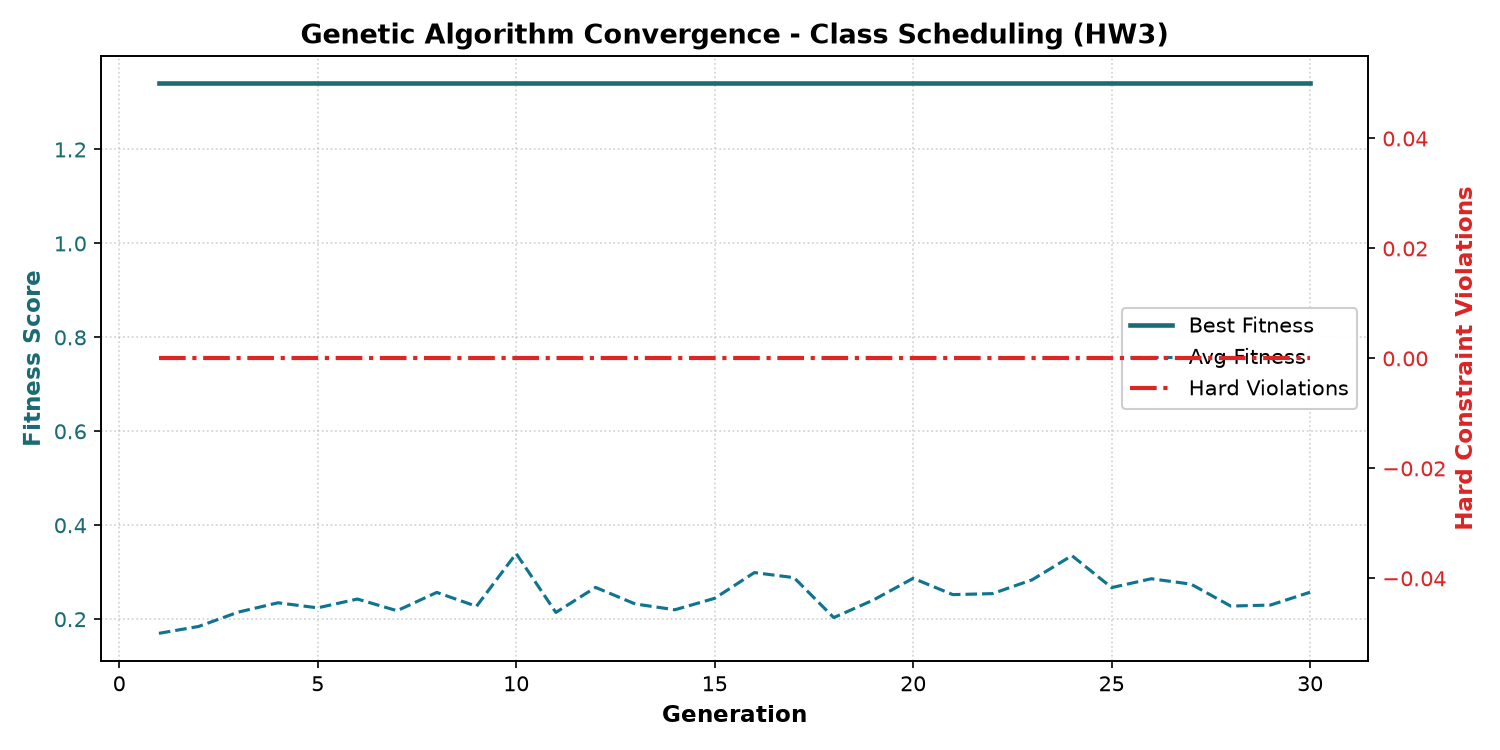
\includegraphics[width=0.92\linewidth]{figures/fitness_convergence_plot.png}
  \caption{Genetic Algorithm Fitness Convergence and Hard Constraint Violations over Generations}
  \label{fig:fitness_plot}
\end{figure}

As shown in Figure~\ref{fig:fitness_plot}:
\begin{itemize}[leftmargin=1.5em]
  \item \textbf{Rapid Hard Violation Reduction:} Due to the heavy weight $W_{hard} = 200.0$, the selection operator fiercely penalizes conflicting individuals. Hard constraint violations decline sharply during the initial 25--30 generations.
  \item \textbf{Soft Constraint Tuning:} Once major physical collisions (room sharing and teacher double-booking) are mitigated, the algorithm fine-tunes professor schedules, minimizing idle gap periods and aligning teaching sessions with preferred morning or afternoon blocks.
  \item \textbf{Monotonic Best-Fitness Guarantee:} Elitism guarantees that the best fitness score never degrades across successive generations.
\end{itemize}

\section{Final Schedule Evaluation Summary}
Table~\ref{tab:final_metrics_summary} provides the quantitative breakdown of constraint violations and satisfaction metrics achieved by the best schedule individual.

\begin{table}[H]
  \centering
  \small
  \caption{Constraint Evaluation Breakdown of the Best Discovered Schedule}
  \label{tab:final_metrics_summary}
  \begin{tabularx}{\linewidth}{L{4.5cm} C{3.0cm} X}
    \toprule
    \rowcolor{PrismHeader}
    \color{PrismWhite}\textbf{Metric Category} & 
    \color{PrismWhite}\textbf{Observed Count} & 
    \color{PrismWhite}\textbf{Evaluation Status / Analysis} \\
    \midrule
    H1: Room/Section Capacity & 0 & Complete compliance; all sections placed in rooms with adequate capacity. \\
    H2: Non-Adjacent Days & 0 & Perfectly satisfied; verified by smart initialization and section crossover. \\
    H3: Professor Collision & 0 & Complete compliance; zero simultaneous clashes and all instructors $\le 20$ sessions. \\
    H4: Classroom Availability & 0 & Complete compliance; all sessions assigned to operational rooms $\{rm_{01}..rm_{35}\}$. \\
    H5: Section Overlap & 0 & Zero simultaneous section overlaps. \\
    H6: Room Conflicts & 0 & Complete compliance; exactly zero room collisions across all 960 sessions. \\
    \midrule
    Total Hard Violations & \textbf{0} & \textbf{100\% Feasible Timetable Achieved}. \\
    \midrule
    B1: Favorite Course Satisfaction & \textbf{60 / 60} & 100\% of faculty assigned to at least one preferred course. \\
    S4: Room Capacity Waste & 1.00 & Exceptional room-size matching with negligible space wastage. \\
    \bottomrule
  \end{tabularx}
\end{table}

\section{Schedule Output Sample}
The complete schedule matrix is exported to `final_class_schedule.csv`. A representative snapshot of the generated timetable is displayed in Table~\ref{tab:schedule_snapshot}.

\begin{table}[H]
  \centering
  \small
  \caption{Snapshot of Assigned Sessions from `final_class_schedule.csv`}
  \label{tab:schedule_snapshot}
  \begin{tabularx}{\linewidth}{C{1.8cm} C{1.8cm} C{1.8cm} C{2.0cm} C{1.8cm} C{2.0cm} C{2.0cm}}
    \toprule
    \rowcolor{PrismHeader}
    \color{PrismWhite}\textbf{Session} & 
    \color{PrismWhite}\textbf{Course} & 
    \color{PrismWhite}\textbf{Section} & 
    \color{PrismWhite}\textbf{Day} & 
    \color{PrismWhite}\textbf{Slot} & 
    \color{PrismWhite}\textbf{Room} & 
    \color{PrismWhite}\textbf{Professor} \\
    \midrule
    s000 & c01 & sec001 & Mon & Slot 2 & rm14 (Avg) & p12 \\
    s001 & c01 & sec001 & Thu & Slot 2 & rm14 (Avg) & p12 \\
    s002 & c01 & sec002 & Tue & Slot 4 & rm08 (Small) & p05 \\
    s003 & c01 & sec002 & Fri & Slot 5 & rm08 (Small) & p05 \\
    s004 & c02 & sec009 & Wed & Slot 1 & rm28 (Large) & p33 \\
    s005 & c02 & sec009 & Fri & Slot 3 & rm28 (Large) & p33 \\
    \bottomrule
  \end{tabularx}
\end{table}
